\section{转动参考系}\label{sec:12.02}


现在,我们选择一个相对于惯性系作转动运动的物体为一新
\begin{wrapfigure}[7]{r}{11em}
    %\vspace{-4em}
    \centering
    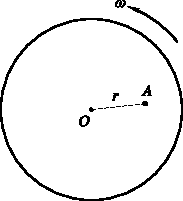
\includegraphics{figure/fig12.03}
    \caption{转动参考系}
    \label{fig:12.03}
\end{wrapfigure}
的参考物。这样一个参考系称为转动
参考系,也是一种非惯性系。因为地球
参考系是个转动参考系,所以关于转
动参考系的问题有特别的实际兴趣。
如上节指出,只要引入相应的惯性
力,则牛顿第二定律可以照用。关于
转动参考系的惯性力,是个较复杂的
问题。下面就几个特定情况来讨论。

% 356.jpg
如图\ref{fig:12.03}所示,图中圆盘以角速度$ \omega $对一惯性系$ K $作匀速转
动。如果质量为$ m $的质点$ A $对于圆盘参考系$ K' $是不动的,即在$ K' $
系看来$ A $是静止的,则应有
\begin{equation*}
    \vec{F} _ \text{总} = 0
\end{equation*}
\begin{align}\label{eqn:12.02.01}
    \beforetext{或} \vec{F} _ \text{真} + \vec{F} _ {in} = 0
\end{align}
在惯性系$ K $中看来,质点$ A $是作以$ r $为半径的匀速圆周运动,它
具有向心加速度$ \omega ^ 2 r $,作用在$ A $上的真实力是向心力$ \vec{F} _ \text{真} $,其大小
应为\vspace{-1.7em}
\begin{equation}\label{eqn:12.02.02}
    | \vec{F} _ \text{真} | = F _ \text{真} = m \omega ^ { 2 } r
\end{equation}
在牛顿力学中,我们总是认为,对不同参考系而言,真实力和质
量是不变的,故由式\eqref{eqn:12.02.01}和式\eqref{eqn:12.02.02}得知,在$ K' $中,$ A $所
受的惯性力$ \vec{F} _ {in} $的大小应为
\begin{equation}\label{eqn:12.02.03}
    F _ { in } = m \omega ^ { 2 } r
\end{equation}
其方向应在离心的方向。因此,称$ \vec{F} _ {in} $为惯性离心力。

惯性离心力的作用在日常生活中是熟悉的。当汽车转弯时,
\begin{wrapfigure}[9]{r}{11em}
    \centering
    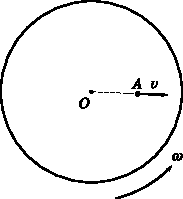
\includegraphics{figure/fig12.04}
    \caption{转动参考系中的直线运动}
    \label{fig:12.04}
\end{wrapfigure}
乘客感到向外甩。这个现象在地面上
的人看来,是因为当汽车转弯时,乘
客仍按惯性定律保持着直线运动,结
果乘客相对于车厢的运动就是向外甩
出。而在车厢参考系看来,乘客的外
甩是由于惯性离心力的作用。

再讨论另一个特殊情况:质量为
$ m $的质点$ A $相对于圆盘参考系$ K' $沿着
半径方向作匀速直线运动(图\ref{fig:12.04}),
根据牛顿力学,从$ K' $系看来,
\begin{equation*}
    \vec{F} _ \text{真} + \vec{F} _ {in} = 0
\end{equation*}
\begin{align*}
    \beforetext{或}\vec{F} _ {in} = - \vec{F} _ \text{真}
\end{align*}
因此,要求出$ A $所受的惯性力$ \vec{F} _ {in} $,只要求得真实力$ \vec{F} _ \text{真} $就可以

\noindent 了。
% 357.jpg
而$ \vec{F} _ \text{真} $在不同参考系中是相同的,所以我们可在惯性系$ K $中求$ \vec{F} _ \text{真} $。
在K中看来,
\begin{equation*}
    \vec{F} _ \text{真} = m \vec{a}
\end{equation*}
$\vec{a}$是质点$ A $相对于$ K $的加速度。所以只要求出加速度$\vec{a}$,就可推知
\begin{equation*}
    \vec{F} _ {in} = - m \vec{a}
\end{equation*}

现在来求$\vec{a}$,假定在$ t $时刻圆盘相对$ K $系的位置如图\ref{fig:12.05a}所
示,质点$ A $相对圆盘参考系$ K' $的速度是$\vec{v}$,而圆盘$ A $处相对$ K $的速
度是$\vec{v}_c$,其大小为$  v _ { c } = \omega r   $。
按速度合成公式,质点$ A $相对于$ K $的速度
是$ \vec{v}+\vec{v}_c $。在$  t + \Delta t  $ 时,圆盘转动到图\ref{fig:12.05b}所示的位置,转
过角度$  \Delta \varphi = \omega \Delta t   $,这时质点$ A $相对于$ K' $的速度是$ \vec{v}' $,由于$ A $相对
于圆盘是匀速直线运动,所以$ \vec{v} ' $在径向$\vec{r}'$的方向,其大小为$  v ^ { \prime } = v $;
现在圆盘$ A $处的速度是$ \vec{v} _ c ^ \prime $,其大小为$  v _ c ^ { \prime } = \omega r ^ { \prime } , r ^ { \prime } = r + v \Delta t $,故质
点$ A $相对于$ K $的速度为$ \vec{v} _ c ^ \prime + \vec{v} ^ \prime $。\vspace{-0.5em}
\begin{figure}[h]
    \centering
    \subfigure[\label{fig:12.05a}]{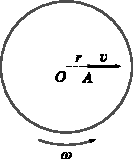
\includegraphics{figure/fig12.05a}}\qquad
    \subfigure[\label{fig:12.05b}]{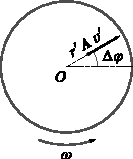
\includegraphics{figure/fig12.05b}}\qquad
    \subfigure[\label{fig:12.05c}]{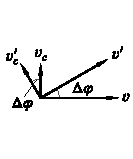
\includegraphics{figure/fig12.05c}}
    \caption{推求科里奥利力}
    \label{fig:12.05}
\end{figure}

根据定义,质点$ A $在$ K $中的加速度为
\begin{equation*}
    \vec{a} = \lim _ { \Delta t \to 0 } \frac { ( \vec{v} _ { c } ^ { \prime } + \vec{v} _ { \prime } ) - ( \vec{v} _ { c } + \vec{v} ) } { \Delta t }
\end{equation*}
下面我们将$ a $分解成平行于$\vec{v}$方向的分量$ a _ {//} $及垂直于$\vec{v}$的分量$ a _ \bot $。
根据图\ref{fig:12.05c},有\\
\begin{equation}\label{eqn:12.02.04}
        \begin{aligned}
    a _ { // } &= \lim_{ \Delta t \to 0 } \frac { v _ { c// } ^ { \prime } + v _ { // } ^ { \prime } - v _ { c// } - v _ { // } } { \Delta t } \\
       &=\lim _{\Delta t \to 0} \frac{-v_{c}^{\prime} \sin \Delta \varphi+v^{\prime} \cos \Delta \varphi-0-v}{\Delta t} \\
        &=\lim _{\Delta t \to 0} \frac{-\omega(r+v \Delta t) \Delta \varphi+v-v}{\Delta t} \\
        &=-\omega^{2} r
    \end{aligned}
\end{equation}
\begin{equation}\label{eqn:12.02.05}
    \begin{aligned}
        a_{\bot} &=\lim _{\Delta \rightarrow 0} \frac{v_{c \bot}^{\prime}+v_{\bot}^{\prime}-v_{c \bot}-v_{\bot}}{\Delta t} \\
        &=\lim _{\Delta \rightarrow 0} \frac{v_{c}^{\prime} \cos \Delta \varphi+v^{\prime} \sin \Delta \varphi-v_{c}-0}{\Delta t} \\
        &=\lim _{\Delta t \rightarrow 0} \frac{\omega(r+v \Delta t)+v \Delta \varphi-\omega r}{\Delta t} \\
        &=+2 v \omega
    \end{aligned}
\end{equation}
$ a_{//} $式中的负号,表示加速度方向与$\vec{v}$方向相反,指向圆心。$ a_{\bot} $式
的正号,表示它的方向垂直于$\vec{v}$向上。现在分别讨论与 $ a_{//}, a_{\bot}$所
相应的惯性力。

与$ a_{//} $相应的惯性力$ F_{//in} $大小为$ m\omega ^ 2 r $,方向平行于$\vec{v}$,也就是
平行于$\vec{r}$。这就是前面讨论过的惯性离心力。惯性离心力的大小
决定于质点距盘心距离$ r $,方向总是离心。无论质点相对于圆盘
运动还是静止,它所受到的惯性离心力都是一样的。

与$ a _ { \bot } $ 相应的惯性力$ F_{\bot in} $的大小是$ 2mv\omega $,如按图\ref{fig:12.05c}的方
位,这个力的方向是垂直于$\vec{v}$向下。这种新类型的惯性力,按照
它的发现者,被命名为科里奥利力。科里奥利力的特点是与质点
对圆盘参考系$ K' $的运动速度有关,当$  \vec{v} = 0   $,即相对于$ K' $静止时,
科里奥利力为零,所以只有对$ K' $运动着的物体才感受到科里奥利
力的作用。再则,科里奥利力与$\vec{v}$的方向垂直,总是力图改变质
点在$ K' $系中的运动方向。

可以一般地证明,在转动参考系中,只有惯性离心力及科里
奥利力这两种类型的惯性力。惯性离心力总可以表示为
% 359.jpg
\begin{equation}\label{eqn:12.02.06}
    \vec{F} _ \text{离} = m \omega ^ { 2 } \vec{R}
\end{equation}
其中矢量$\vec{R}$的大小为质点$ A $到转轴的距离,方向由转轴沿径向指向质点$ M $。科里奥利力总可以表成
\begin{equation}\label{eqn:12.02.07}
    \vec{F} _ { c } = 2 m \left( \vec{v} \times \vec{\omega} \right)
\end{equation}
其中$\vec{v}$是质点$ A $相对于$ K' $的速度;$\vec{\omega}$是参考系$ K' $的转动角速度矢
量。

地球是一个转动参考系,上述两种惯性力的效果在地球上都
有反映,有很大的实用意义。我们首先看一种简单情况,物体相
对于地球静止。由于地球是一个以$ \omega $匀速转动的参考系,质量为
$ m $的静止在地球表面的物体,在地球参考系观察者看来,必定受
到惯性离心力$ \vec{F}_\text{离} $,其大小为$  \omega ^ { 2 } R   $,$ R $是物体到地球自转轴的距
离,力的方向为沿径向$ R $向外,如图12.6所示。显然,当纬度不
\begin{wrapfigure}[11]{r}{11em}
    \centering
    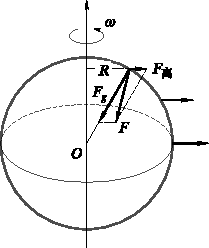
\includegraphics{figure/fig12.06}
    \caption{地球上物体所受到的惯性离心力}
    \label{fig:12.06}
\end{wrapfigure}
同时,$ \vec{F}_\text{离} $不同,两极处最小
为零;赤道处最大。地球上的自
由落体要受到$ \vec{F}_\text{离} $和地球引力$ \vec{F}_g $
两方面的作用。很容易看出,在
不同纬度,上述两力的合力大小
是不等的,因此,即使地球真是
均匀的球体,各处的重力加速度
也并不相同,极区大,赤道处
小。惯性离心力是造成各处$ g $不
等的重要原因之一。此外,我们
习惯说,用线悬挂一物体,则当
相对于地球静止时,悬线指向地心。其实,这个说法也并不严格。
绳应静止在$ \vec{F}_\text{离} $和$ \vec{F}_g $的合力$ \vec{F} $的方向。从图\ref{fig:12.06} 上可以看出,
$ \vec{F}_g $指向地心,而$ \vec{F} $并不指向地心,且这种偏离在不同纬度上有不
同值。

现在讨论科里奥利力的一些效应。当质量为$ m $的质点相对于
% 360.jpg
地球以$\vec{v}$运动时,必定要受到科里奥利力的作用,它由式 \eqref{eqn:12.02.07}
所描写。由式\eqref{eqn:12.02.07}不难断定,无论质点向哪方向运动,在北
半球,$ \vec{F}_c $总是指向质点行进方向的右侧;而在南半球,$ \vec{F}_c $总是
指向质点行进方向的左侧。北半球的河流总是冲刷右岸,使河床
大都是右岸陡,左岸坡单行的火车轨道,总是右边的铁轨比左
边的铁轨要磨损得重些。上述诸现象在南半球则相反,这些都是
科里奥利力的作用。地球上很多左右不平衡的现象都与科里奥利
力有关。

科里奥利力的存在,是对地球相对于惯性系有转动的一个严
格的物理证明。直接证明地球参考系中存在科里奥利力的物理实
验是佛科摆。佛科摆是一个普通的单摆,只不过顶端的连接装置
保证悬点能在任何方向上同样自由地摆动。如图\ref{fig:12.07} 所示。如果
地球是惯性系,不论摆动多久,摆总是在同一个平面内,因为不
存在侧向力。如果地球是转动着的非惯性系,摆锤将受到侧向的
科里奥利力。在北半球,这个力总是指向右侧。图\ref{fig:12.07} 是由上向
下看的摆锤的轨道,当摆锤从1走向2时,不是沿直径到$ 2' $,而
是向右偏到达2,从2向3时,不是沿直径到达$ 3' $,而是到达
3,如此等等,就会使摆平面转动。1851年,佛科在巴黎的伟人
祠内大圆屋顶下公开表演了这个实验,看到了摆平面的转动。由
摆平面的转动,我们能严格地求得地球相对惯性系的转动角速度。可

\begin{figure}[h]
    \begin{minipage}[b]{0.5\linewidth}
        \centering
        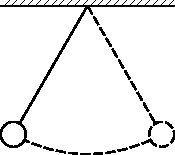
\includegraphics{figure/fig12.07}
        \caption{佛科摆}
        \label{fig:12.07}
    \end{minipage}
    \begin{minipage}[b]{0.5\linewidth}
        \centering
        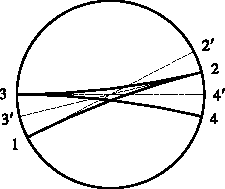
\includegraphics{figure/fig12.08}
        \caption{佛科摆锤轨道}
        \label{fig:12.08}
    \end{minipage}
\end{figure}% 361.jpg
\noindent
以说,直到这时,才算真正把亚里士多德的地心说与哥白
尼的日心说之争分清了。

\example 如图\ref{fig:12.09a}所示,用长为$ l $的绳将质量为$ m $的小球
悬挂起来,令物体以匀速率$ v $沿一水平圆周运动。物体运动时,
绳与竖直方向的夹角$ \theta $不变。这个装置称为圆锥摆。试求此圆锥
摆的周期$ T $。

\begin{figure}[h]
    \centering
    \subfigure[\label{fig:12.09a}]{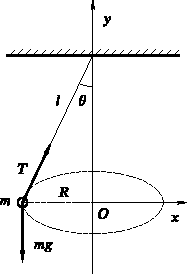
\includegraphics{figure/fig12.09a}}\qquad
    \subfigure[\label{fig:12.09b}]{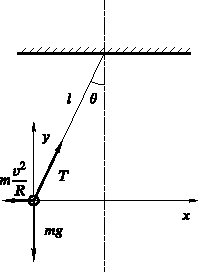
\includegraphics{figure/fig12.09b}}
    \caption{}
    \label{fig:12.09}
\end{figure}

\solution 可以从两种参考系来解这个题。一为地面惯性系,在此,
摆锥受两个力的作用,即张力$ T $及重力$ mg $;二是随$ m $一起运动的
参考系,此为旋转系,在此,摆锤受三个力的作用,即张力$ T $、
重力$ mg $及惯性力$ mv^2/R $。在惯性系中,$ m $作圆周运动;在旋转系
中,$ m $静止不动。用两种观点可解出同样的结果。下面分别求解

(1) 惯性系解法。取坐标如图\ref{fig:12.09a},它是一个圆锥摆。
故有
\begin{align*}
    T _ { y } &= T \cos \theta = m g \\
    T _ { x } &= T \sin \theta = m v ^ { 2 } / R \\
    R &= l \sin \theta
\end{align*}
% 362.jpg
将上三式联立求解,得
\begin{equation*}
    v = \sqrt { R g \tg \theta }
\end{equation*}
周期则为
\begin{align*}
    T &= \frac { 2 \uppi R } { v } \\
      &= 2 \uppi \sqrt{ \frac { l \cos \theta } { g }}
\end{align*}

(2) 非惯性系解法。此时处理的是一个静力平衡的问题,坐
标原点取在$ m $上,$ x $与$ R $重合,$ oy $是竖直方向,如图\ref{fig:12.09b}所
示。张力、重力$ mg $及惯性力$ mv^2/R $三力平衡即为
\begin{align*}
    T \cos \theta &= m g \\
    T \sin \theta &= m v ^ { 2 } / R \\
    R &= l \sin \theta
\end{align*}
结果与上面相同。

\example 使长为$ l $的细绳一端固定在以匀速转动的水平光
\begin{wrapfigure}[8]{r}{13em}
    \centering
    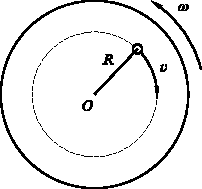
\includegraphics{figure/fig12.10}
    \caption{}
    \label{fig:12.10}
\end{wrapfigure}
滑圆盘在中心$ O $点上,绳的另一
端系一质量为$ m_0 $的小球。欲使小
球在盘上相对于盘以匀速率$ v $作
圆周运动,旋转方向与盘相反。
问绳中的张力$ T $多大?

\solution (1) 惯性系解法。小球
受绳的张力$ T $是向心力,使小球
产生向心加速度,此为相对于地
面的绝对加速度$ a_\text{绝对} $:
\begin{align*}
    T _ { T } &= m a_\text{绝对} \\
    a_\text{绝对} &= \frac { v _\text{绝对} ^ { 2 } } { l }
\end{align*}

% 363.jpg
\clearpage
\begin{align*}
    \beforetext{因为} \vec{v}_\text{绝对} = \vec{v}_\text{相对} + \vec{v}_\text{牵连}
\end{align*}
\begin{align*}
    \beforetext{所以} v_\text{绝对} &= v - l \omega \\
    a_\text{绝对} &= \frac { \left( v - l \omega \right) ^ { 2 } } { l } \\
                 &= \frac { v ^ { 2 } } { l } + l \omega ^ { 2 } - 2 v \omega \\
            T &= m \frac { v ^ { 2 } } { l } + m l \omega ^ { 2 } - 2 m v \omega
\end{align*}

(2) 非惯性系解法。小球受到绳的张力与惯性力的合力为向
心力,使它作匀速率$ v $的圆周运动。此时要用到在非惯性系中的
相对加速度。

在旋转坐标系中,作匀速圆周运动的物体受到两个惯性力的
作用,即惯性离心力($ f' $)
\begin{equation*}
    - m \frac { v _\text{牵连} ^ { 2 } } { l } = - m l \omega ^ { 2 }
\end{equation*}
和科里奥利力($ f'' $)
\begin{align*}
    &2 m v \omega \\
    \beforetext{所以} &\vec{T} + \vec{f} ^ { \prime } + \vec{f} ^ { \prime \prime } = m \vec{a} _ \text{相对} \\
   \beforetext{即} &T + 2 m v \omega - m l \omega ^ { 2 } = m \frac { v ^ { 2 } } { l } \\
   \beforetext{故} &T = m \frac { v ^ { 2 } } { l } + m l \omega ^ { 2 } - 2 m v \omega
\end{align*}
与上述结果相同。